\begin{landscape}
\section{Data Description}
\begin{center}
\begin{longtable}{l | p{5cm} | p{1.5cm} | p{10cm}}
\label{tab:data}
No & Data Source &	Data Origin	& Description \\
\hline
1 &	F1 data, 2 csv files	& provided & \\
2 &	F2 data,  5 csv files	& provided &	49092 rows, 0-211 cycles, 44 var, Initial fermentation data \\
3 & F4 data, 7 csv files	& provided &	49092 rows, 0-213 cycles, 60 var, yeast product data \\
4 &	F5 data, 6 csv files	& provided &	49093 rows, 0-282 cycles, 52 var, Commercial yeast product data \\
5 &	F7 data, 6 csv files	& provided &	49092 rows, 0-225 cycles, 52 variables \\
6 &	F8 data, 6 csv files	& provided &	49092 rows, 0-135 cycles, 52 variables\\
7 & CSep data, 3 csv files	&provided \\	
8 &	MO data, 17 csv files	&provided \\	
9 &	Seps data, 9 csv files	&provided \\	
10&	SR data, 11 csv files	&provided \\
11&	Manual fermentation recordings,  
F2-F4 10 pdf, F5 2 pdf files&	provided&	processes manually filled in pdf. Data contains only F4 and F5 fermentations recordings  \\
12&	Brown colonies ferms, word doc
(Quality control results for few F4 and F5 batches)	&provided&	Data has attributes
\begin{itemize}
    \item Production Date (MM-DD-YYYY) -finished product date
    \item Strain (yeast strain no 7442 only)
    \item Seed - batch number
    \item Commercial – if F5
    \item Lot no - number of batches
    \item 	Status - quality control decision: Rejected, Released, Restricted release)
\end{itemize} \\
13&	Data Parameters - Excel with fermentation variable details  	&provided&Glossary, some variables description. Mainly variables represent a specified volume or mass of ingredients from yeast manufacturing formulas, also process condition measurements, such as an air or water temperatures, etc.\\

14&	Labelled Dataset - samples with statuses 
\begin{itemize}
    \item F2 samples: 1469 obs. of 45 variables
    \item F4 samples: 1252 obs. of 62 variables
    \item F5 samples: 294 obs. of 54 variables
\end{itemize}
&created& 	
Based on provided manual notes and quality control results.  
For few F2, F4 and F5 data there were manually assigned labels (statuses): \begin{itemize}
    \item REJECT
    \item RELEASE
    \item RESTRICT
\end{itemize}
\\
\hline
\end{longtable}
\end{center}
\end{landscape}

\section{Correlation plots of the parametric data}

\begin{figure}[ht]
    \centering
    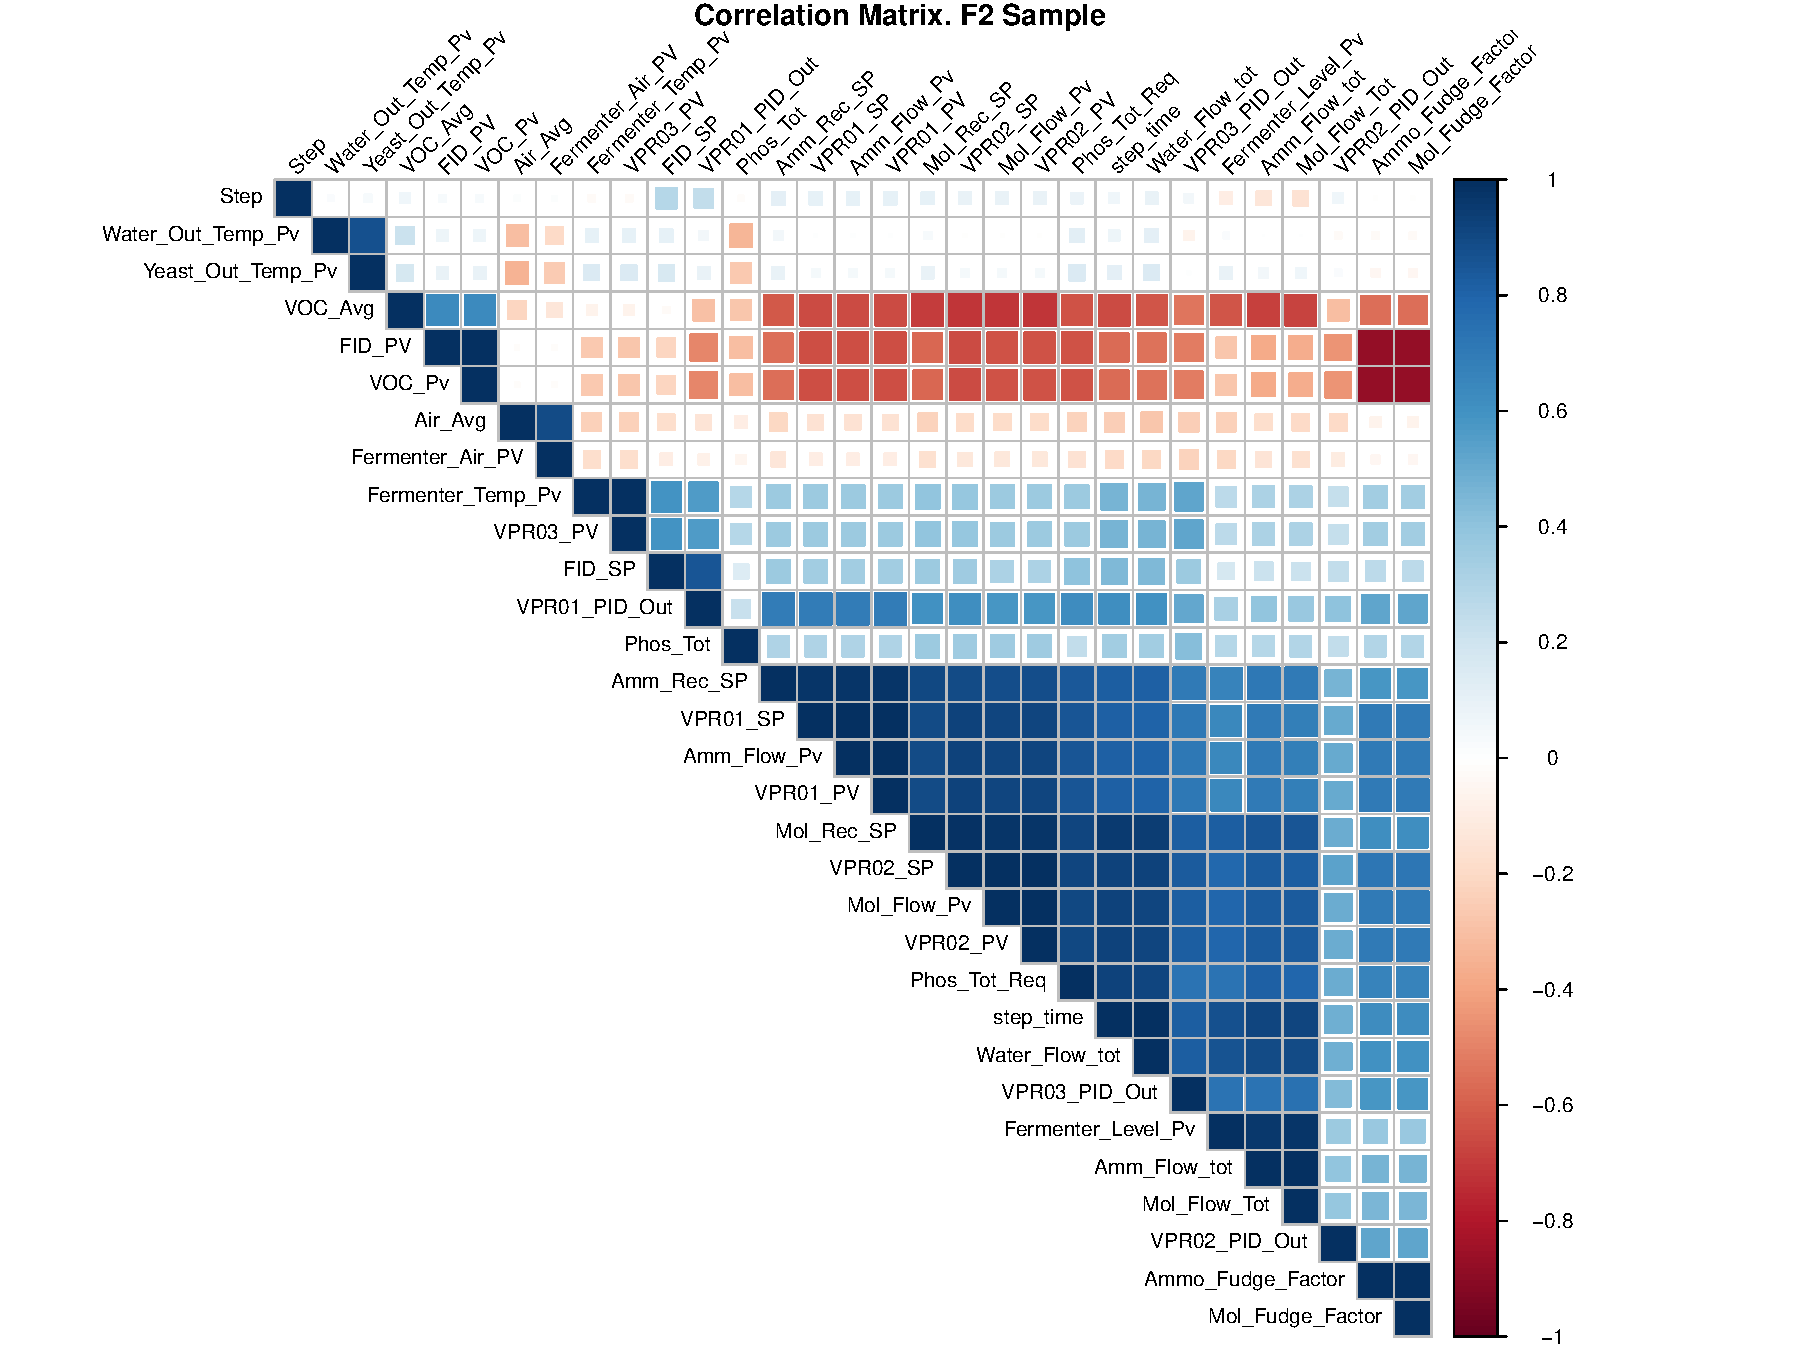
\includegraphics[width=1\textwidth]{plots/f2_correlation.pdf}
    \caption{F2 correlation matrix}
    \label{fig:f2_correlation}
\end{figure}

\begin{figure}[ht]
    \centering
    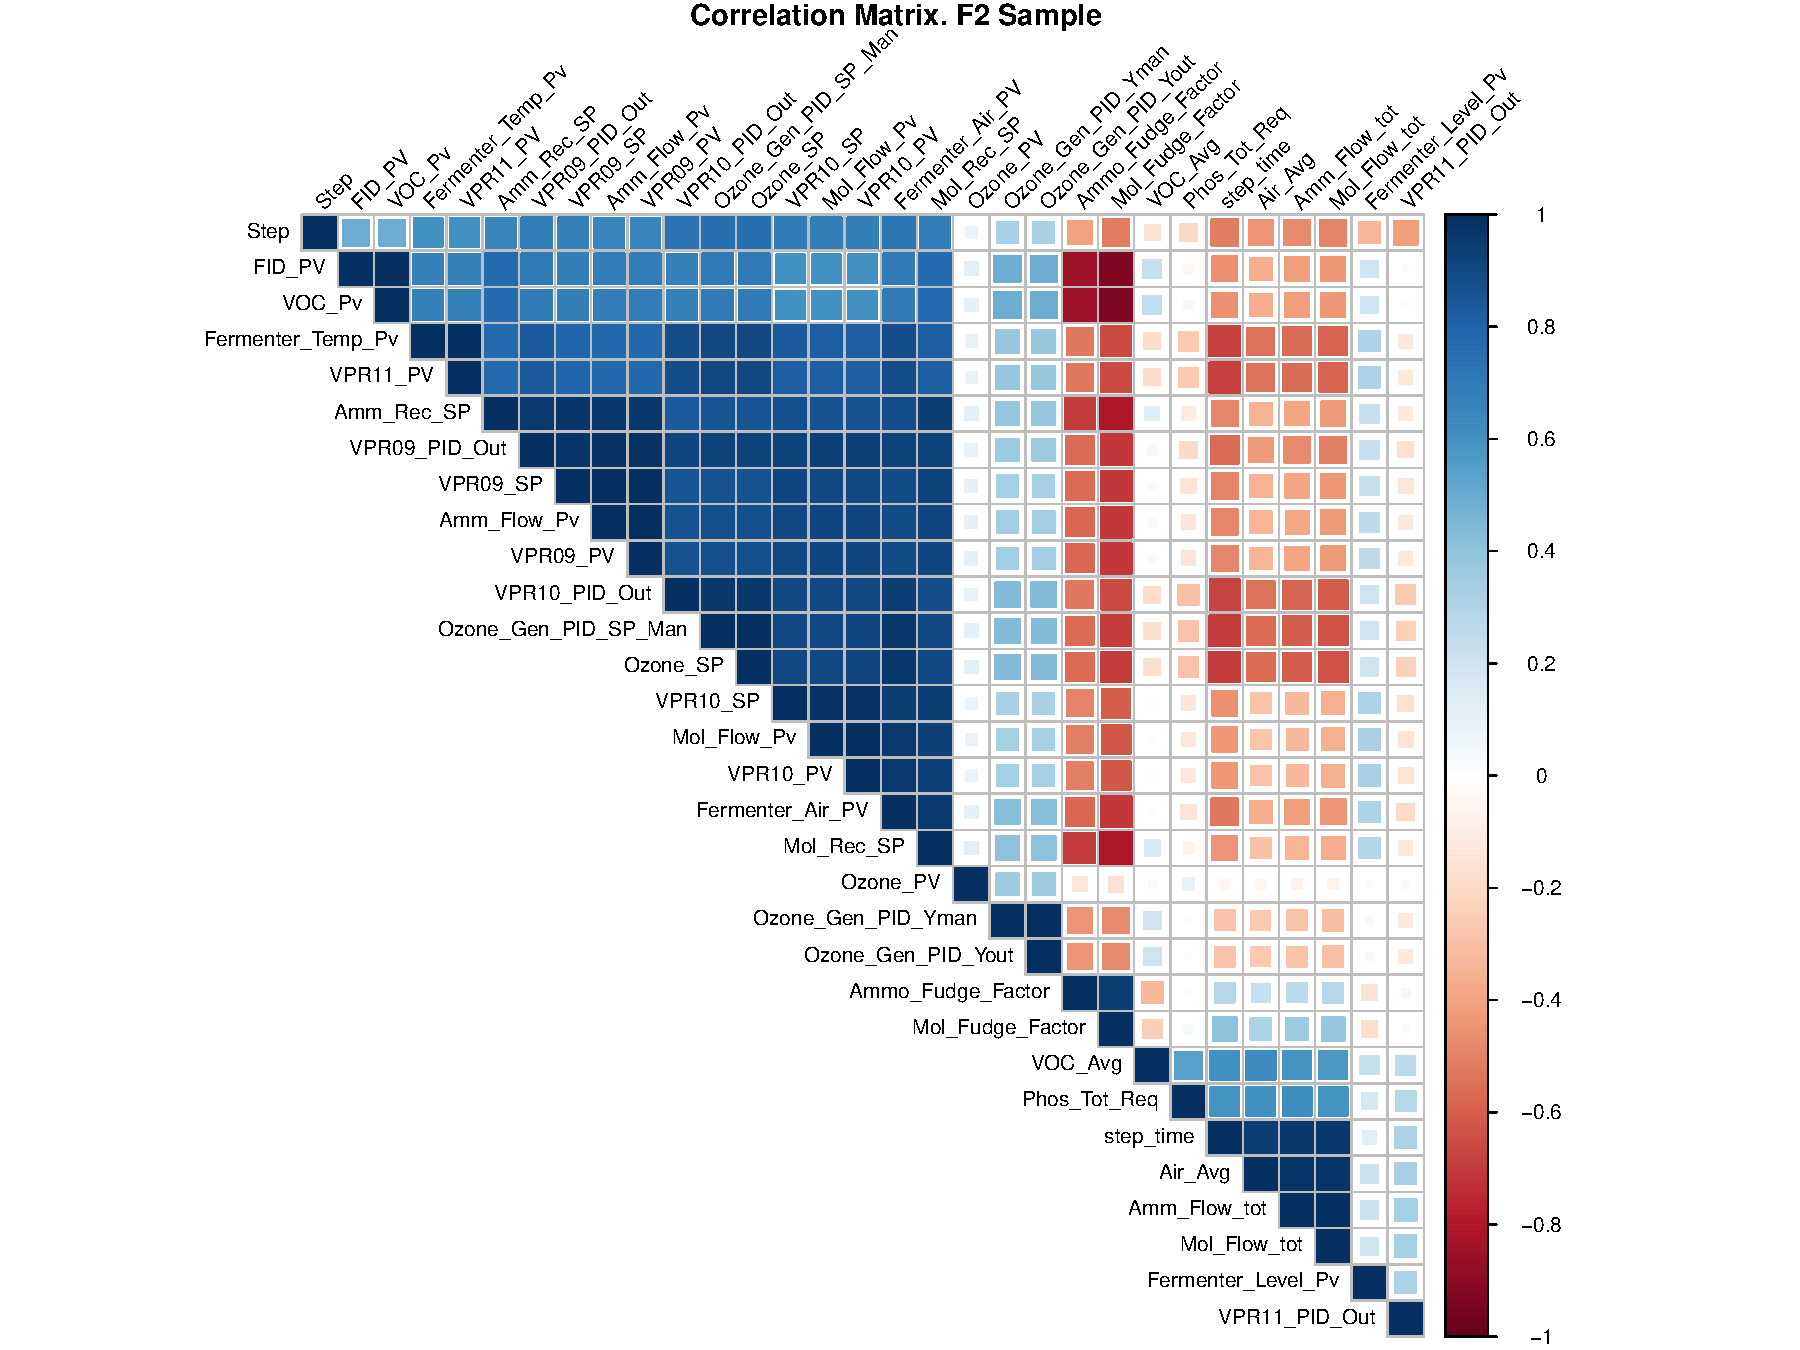
\includegraphics[width=1\textwidth]{plots/f4_correlation.pdf}
    \caption{F4 correlation matrix}
    \label{fig:f4_correlation}
\end{figure}

\begin{figure}[ht]
    \centering
    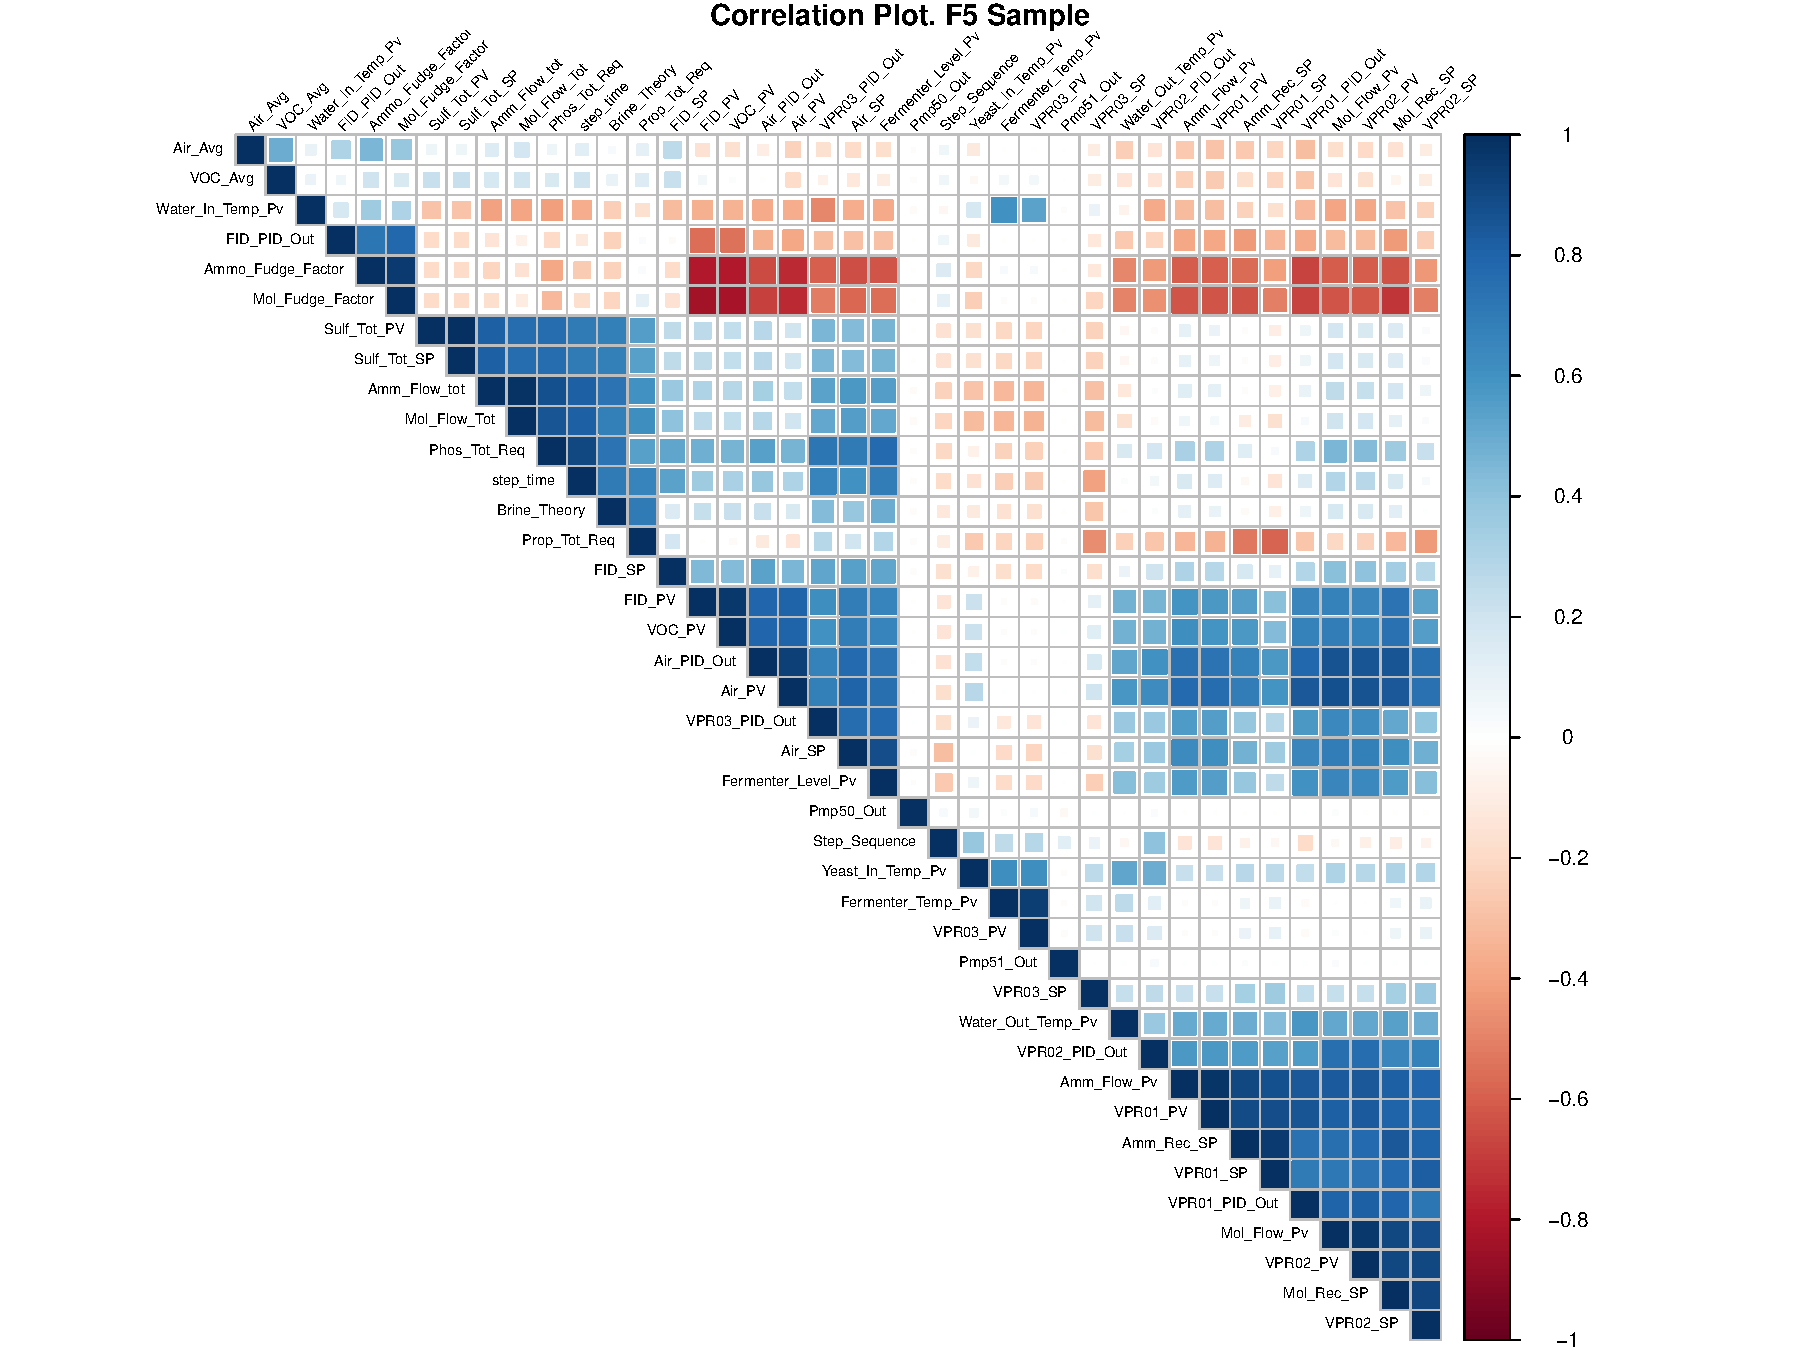
\includegraphics[width=1\textwidth]{plots/f5_sample_correlation.pdf}
    \caption{F5 correlation matrix}
    \label{fig:f5_correlation}
\end{figure}


